\documentclass[a4paper,12pt,headsepline]{scrartcl}


\usepackage{biblatex}
\addbibresource{main.bib}

\usepackage[bookmarksnumbered, hyperfootnotes=false]{hyperref}
\usepackage{xurl} % break long URLs
\usepackage[margin=1in]{geometry}
\usepackage[T1]{fontenc} % correctly typesetting characters and symbols
\usepackage[shortlabels]{enumitem} % for \begin{itemize} [$\circ$]
\usepackage[table]{xcolor}
\usepackage{lmodern} % font
\usepackage{graphicx}
\usepackage{standalone} % to import Tikz figures from standalone documents
\usepackage{tikz}
\usetikzlibrary{arrows.meta, positioning, shapes, snakes, fit, calc, patterns}
\usepackage{amsmath}
\usepackage{algorithm}
\usepackage{algorithmic}
\usepackage{mathtools}
\usepackage{enumerate}
\usepackage{centernot} % f.e. to write "not a subset of"
\usepackage{longtable}
\usepackage{fancybox}
\usepackage{color}
\usepackage{amssymb}
\usepackage{array}
\usepackage{multirow}
\usepackage{bm}
\usepackage{amsthm}
\usepackage{cleveref} % use Cref to automatically add "Figure", "Section", or "Table" in front of the reference
\usepackage{caption}
\usepackage{subcaption}

\usepackage{scrlayer-scrpage}
\pagestyle{scrheadings}
\clearpairofpagestyles %
\chead{\leftmark\hfill\pagemark}
\DeclareMathOperator*{\argmax}{arg\,max}
\DeclareMathOperator*{\argmin}{arg\,min}

% https://www.overleaf.com/learn/latex/Theorems_and_proofs
\theoremstyle{definition}
% \newtheorem{definition}{Definition}[section]
\newtheorem{definition}{Definition}
\newtheorem{theorem}{Theorem}
\theoremstyle{remark}
% \newtheorem*{remarkdf}{remarkdf}
\newtheorem{remarkdf}{Remark}[definition]
\newtheorem{remarkth}{Note}[theorem]

\hyphenation{
    align-ments
}


\begin{document}

\thispagestyle{empty}

\hrule
\vspace{0.5cm}
\begin{center}
    {\huge \bfseries Title}
    \vspace{0.5cm}
    \hrule
    \vspace{0.4cm}
    \today
\end{center}
\newpage

\pagenumbering{roman}
\section*{Abstract}
\addcontentsline{toc}{section}{Abstract}This is the abstract.
\newpage
% \thispagestyle{empty}
\tableofcontents\newpage
\listoffigures
\addcontentsline{toc}{section}{List of Figures}

\listoftables
\addcontentsline{toc}{section}{List of Tables}

\newpage

\pagenumbering{arabic}
\section{First Section}
\markboth{First Section}{}

Text of section 1. Here, a citation is used \cite{sample}.\\
And a long Url nicely wrapped. And a long Url nicely wrapped. And a long Url nicely wrapped.
\url{https://scholar.google.de/scholar?hl=en&as_sdt=0\%2C5&q=GNN+chaos+game+
representation&btnG=&oq=GNN+chaos+game+repre}

\subsection{First subsection}

\begin{table}
    \center
    \begin{tabular}{c|c}
        this   & is    \\\hline
        sample & table \\
    \end{tabular}
    \caption{This is table 1.}
\end{table}

\begin{figure}
    \center
    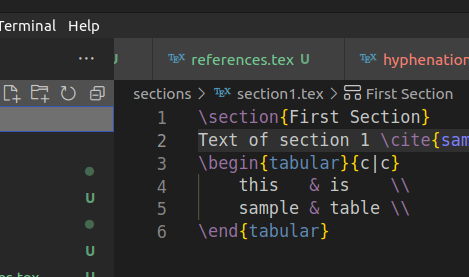
\includegraphics[width=4cm]{fig/images/figure_01.png}
    \caption{This is Figure 1.}
\end{figure}

\begin{figure}
    \center
    \includestandalone{fig/tikz/tikz_figures}
    \caption{This is my tikz figure}
\end{figure}

\newpage
\section{Second Section}
\markboth{Second Section}{}



\newpage
\phantomsection % to make the click in the TOC to forward here instead of the previous section
\markboth{References}{}
\addcontentsline{toc}{section}{References}
\printbibliography

\end{document}